%************************************************
\chapter{Edge-on Talbot-Lau interferometry}\label{ch:edgeon} % $\mathbb{ZNR}$
%************************************************
This chapter is also featured in\cn Thüring T, Abis M, Wang Z, David C,
Stampanoni M, \emph{X-ray phase-contrast imaging at
100 keV on a conventional source.}

\section{Introduction}
High-energy Talbot interferometry has been reported so far using a
synchrotron source at nominal energies of
$\SI{82}{\kilo\electronvolt}$~\cite{Willner2013}. Using a low-brilliance
X-ray tube, Talbot-Lau interferometry was applied so far at
$\SI{60}{\kilo\electronvolt}$ design energy~\cite{Donath2009a}. Medical imaging
applications may benefit from phase contrast at higher energies: chest or
abdominal radiography or \ac{CT} require an acceleration voltage between
\num{100} and $\SI{150}{\kilo\voltpeak}$. Other potential applications are
homeland security or chip failure analysis, which require high energies for
the visualization of materials of high density and atomic number.

\section{Results}
We introduce a method for phase contrast imaging which works on
conventional X-ray sources, covers the entire diagnostic X-ray energy range
and is compatible with compact imaging arrangements. The approach is based
on Talbot-Lau interferometry~\cite{Pfeiffer2006} and employs an edge-on
illumination approach for the grating design and arrangement. Our solution
removes one of the major hurdles which prevented grating interferometry from
being applied at high energies so far, namely the fabrication of gratings
with high aspect ratios. The aspect ratio, given by
\begin{equation}
    \text{R} = \frac{2h}{p},
\end{equation}
where $p$ is the
grating period and $h$ the  structure height, is limited by the
fabrication process, usually photolithography~\cite{David2002} or X-ray
lithography~\cite{Mohr2012} since grating structures tend to collapse or deform
(e.g.\ due to capillary forces) if the aspect ratio is too high.
Moreover, when using a broad spectrum, photons above the design energy
should also be efficiently blocked by the gratings, thus requiring even
higher aspect ratios. The largest aspect ratios achieved by current
fabrication techniques~\cite{David2007,Kenntner2010} are around 60.
For a given setup length these parameters depend on the target energy $E$
according to $p \propto 1/\sqrt{E}$ and $h \propto E^3$, and therefore
$\textnormal{R} \propto E^{7/2}$~\cite{Momose2003a}. If at
$E=\SI{25}{\kilo\electronvolt}$ an aspect ratio for the absorption grating
around $\textnormal{R}=30$ is sufficient, it would have to be at least
$\num{128}$ for $E=\SI{100}{\kilo\electronvolt}$. With our design, we reach
an aspect ratio of \num{143}, satisfying the above condition with a
transmission of less than \SI{1}{\percent} at \SI{100}{\kilo\eV}. As a
comparison, a recent interferometer implemented at a third generation
synchrotron facility~\cite{Willner2013} reported an aspect ratio of
\num{21} with a transmission as large as \SI{20}{\percent}
at~\SI{82}{\kilo\eV}.

Our design introduces edge-on illuminated,  circularly aligned structures.
Edge-on illumination (Fig.~\ref{Fig:schematic}), as
opposed to face-on illumination, exploits the dimension along the grating
lines to form a high aspect ratio of the structures in the direction of the beam. The
effective structure height of the grating is then determined by the grating
dimension along the grating lines, which essentially allows arbitrarily high
aspect ratios. 
\begin{figure}[h!]
    \centering
    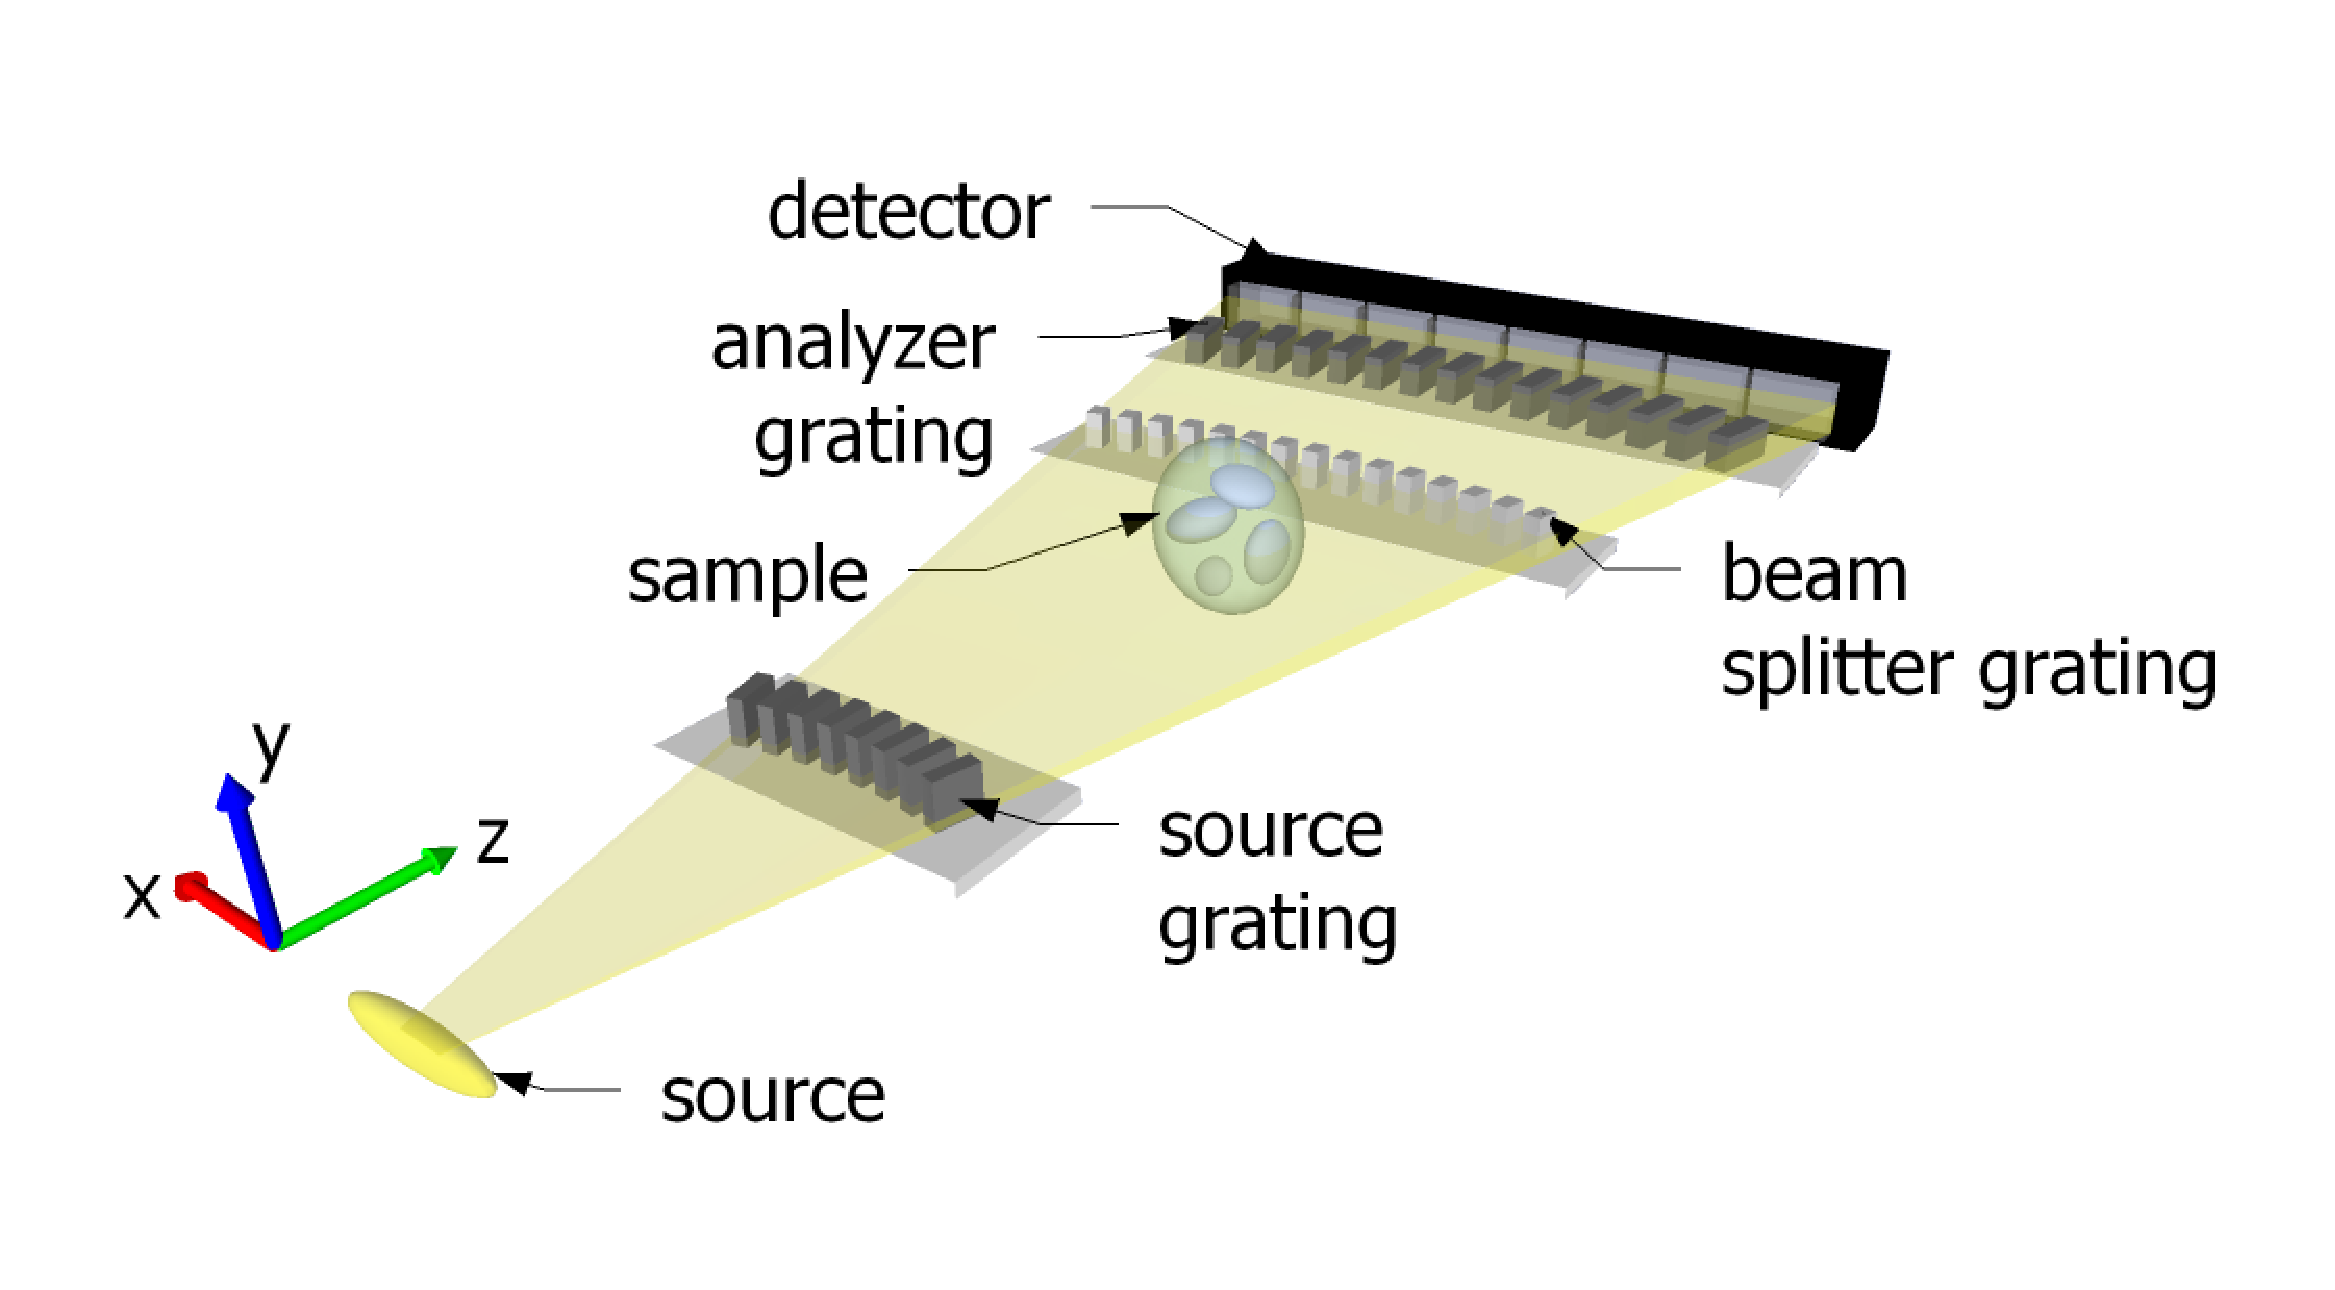
\includegraphics[width=.7\textwidth]{gfx/figure1.eps}
    \caption{Schematic of a grating
        interferometer for X-ray energies between 60 and
        \SI{150}{\kilo\electronvolt} in edge-on illumination mode. The
        aspect ratio is defined by the ratio of the traveling distance along the
        grating lines and the period and can be arbitrarily long. In order to maximize
        the field of view, the grating structures are aligned on an
        arc. A \SI{100}{\kilo\eV} setup was realized where the distance
        between the source and the source grating is \SI{23}{\centi\metre}
    and the distance between the source grating and the phase grating is
    \SI{16}{\centi\metre}. That is also the distance from the phase grating
to the analyzer grating.}%
\label{Fig:schematic}
\end{figure}

Increasing the aspect ratio of the gratings typically leads to a reduction
of the field of view due to the change of the grating transmission function
at high incident angles. In order to overcome this problem, the grating
lines are circularly aligned with a radius equal to the distance to the
source. This allows to achieve an arbitrarily large field of view in a
fan-beam geometry, a significant improvement compared to face-on based and
glancing angle~\cite{Stutman2012a} approaches.

The combination of edge-on illumination and circularly aligned structures
enables phase-contrast imaging at arbitrary design energies and with a
maximum field of view in the horizontal direction ($x$ direction). These
advantages come at the expense of a limited field of view in the vertical
direction ($y$ direction), which is, depending on the X-ray detector,
typically a few pixels. However, radiographic 2D imaging can be obtained by
scanning the sample or a thin fan beam. The scanning technique has been
demonstrated to deliver less dose than the conventional approach based on
the illumination of a large area. In digital mammography, for instance,
where dose is a critical issue, Philips' MicroDose system combines a
scanning approach with an highly collimated fan beam~\cite{Aslund2007}.
Thanks to the high collimation, the dose deposited on  patients has been
reported to be significantly lower than with other instruments based on the
illumination of a large area detector~\cite{Oduko2010}. Similarly, for
tomographic images, the approach allows single slice \ac{CT} or full 3D
imaging in scanning mode.

Grating design and fabrication is nonstandard and involves a complex mask
design, as shown in Fig.~\ref{Fig:grating_mask}. Multiple gratings can reside on a
silicon chip with their specific structure length and curvature. For the
current experiments, a symmetric interferometer with a grating period of $p
= \SI{2.8}{\micro\metre}$ for all gratings has been used. The design energy
is $\SI{100}{\kilo\electronvolt}$ and the beam splitter grating periodically
shifts the phase by zero and $\pi$ at this energy~\cite{David2002}. Using
gold as the phase shifting material, a structure length of
$h_1 = \SI{19.8}{\micro \metre}$ is required. The analyzer grating is an absorption mask
for sensing slight changes of the interference pattern generated by the beam
splitter~\cite{Momose2003a}. With a structure length of $h_2 =
\SI{800}{\micro \metre}$
it can absorb more than \SI{90}{\percent} of the incoming X-rays up to energies of 
$\SI{160}{\kilo\electronvolt}$. The beam splitter and analyzer grating are
separated at the first fractional Talbot order~\cite{Weitkamp2005},
resulting in an intergrating distance of $\SI{158}{\milli\metre}$. However,
the precise position of the analyzer grating along the beam axis is not
critical, and a change in visibility of less than \SI{1}{\percent} is
observed by displacing it by as much as \SI{5}{\milli\metre}. The
source grating splits the relatively large focal spot ($\sim
\SI{1}{\milli\metre}$) into an array of individually coherent, but mutually
incoherent sources~\cite{Pfeiffer2006}. It is also made of gold structures
with a length of $h_0 = h_2 = \SI{800}{\micro \metre}$.
\begin{figure}[h!]
    \centering
    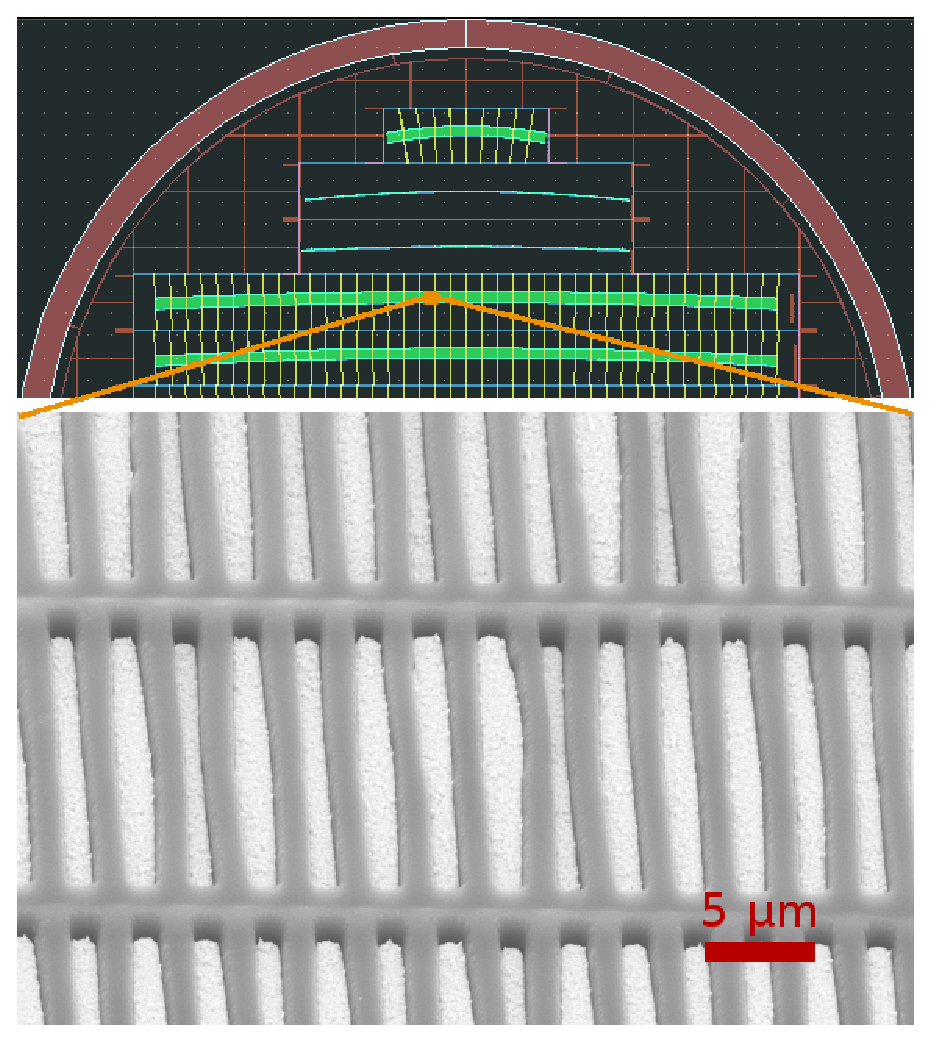
\includegraphics[width=.6\textwidth]{gfx/grating_mask.eps}
    \caption{Grating design mask for
        the edge-on illumination approach and \ac{SEM}
        image of the grating. The top part of the 4 inch wafer shows
        five grating chips. From top to bottom, one source grating, two
        phase gratings and two analyzer gratings. The
        gratings have different curvatures which are specific to the grating
        interferometer geometry. Multiple gratings for more than one setup
        geometry are fabricated on a single wafer.
        The \ac{SEM} image shows the gold structures and the interrupting bridges
        that prevent the lamellae from collapsing~\cite{Kenntner2010}.}\label{Fig:grating_mask}
\end{figure}

Due to the large spectral acceptance~\cite{Weitkamp2005,Thuering2013c} of the
interferometer ($\SI{50}{\kilo\electronvolt}$ to
more than $\SI{160}{\kilo\electronvolt}$) and the high attenuation efficiencies of
the source and analyzer gratings (more than $90\%$ up to
$\SI{160}{\kilo\electronvolt}$), the voltage of the X-ray source was set to
the maximum of $\SI{160}{\kilo\volt}$. With a structure height of
approximately $\SI{100}{\micro \metre}$, the field of view in the vertical
direction is limited to one detector pixel row. In the horizontal direction,
the field of view is only limited by the grating size to
$\SI{30}{\milli\metre}$, but wider gratings can be fabricated with the same
method and the available technology on larger wafers. In addition to the standard components (source,
camera, interferometer), two optical slits, one in front of the source
grating, the other in front of the camera, were required for the collimation
of the beam in the vertical direction. 

Fig.~\ref{Fig:img_chip} shows the first X-ray images acquired with our new setup, based on
edge-on illuminated grating interferometry powered by a conventional X-ray
source operated at \SI{160}{\kilo\voltpeak} and with a design energy of
\SI{100}{\kilo\eV}.  
\begin{figure}[h!]
    \centering
    \includegraphics[width=.5\textwidth]{gfx/images_S00075_S00071.eps}
    \caption{Radiographic scan of an electronic chip. The image was acquired
        with 24 phase steps per line and an exposure time of \SI{15}{\second} per
    step. The top right image shows the differential absorption image.}\label{Fig:img_chip}
\end{figure}
Several resistors and integrated circuits located on different
layers on an electronic chip can be identified. The radiographs were acquired in scanning
mode, using a step size of \SI{100}{\micro\metre} along the $y$ axis, covering a total imaging
area of $2 \times \SI{2}{\centi\metre^2}$. For a better comparison of the magnified phase and
attenuation images, the latter has been replaced with the differential
attenuation image, which was obtained by calculating the derivative along
the horizontal axis. In the attenuation image, the contrast of the soldering
points of the integrated circuit is reduced underneath the resistors, while
in the phase image, they can clearly be identified. The reduced contrast of
the soldering points in the absorption image is due to beam hardening. The
spectrum impinging on these soldering point is hardened by the resistors in
the upper layer, resulting in lower absorption contrast. Due to the weaker
energy dependence of phase shifts ($1/E$ compared to $1/E^3$), phase-contrast
images are less sensitive to beam hardening~\cite{Chabior2011a}, which explains the lower
contrast reduction of the soldering points under the resistors in the
phase image of the chip. This example shows one of the potential benefits of
phase contrast X-ray imaging at high energies, which may be useful to
identify flaws in multilayered structures such as electronic chips.

\section{Discussion}

Possible usages of edge-on grating interferometry encompass applications
ranging from medical imaging to non-destructive testing and homeland
security. All these applications seek for high (greater than
\SI{100}{\kilo\eV}) nominal energies
and compact designs. Particularly for medical application, the operation of
a phase contrast imaging device at high energies is imperative. When imaging
patients, a crucial issue is the dose, which depends mainly on the
absorption of the X-rays and decreases with the third power of the photon
energy~\cite{Momose2005}. On the other hand, the phase interaction is only inversely
proportional to the energy and is therefore relatively much more relevant
than absorption as the energy increases, possibly leading to a decreased
exposure for an equivalent image quality. Clinical operation of such a
device will imply measuring patients who normally breath, move and shake.
Fast acquisitions are therefore required, in order to keep the images sharp
and artifact free. As a consequence, compact, efficient imaging systems need
to be developed to provide imaging capabilities at sufficient speed. Our
circular grating alignment matches the structures of the diffracting and
absorbing elements to the divergent beam, especially for compact geometries.
In conclusion, short, high-energy phase-contrast systems will enable the
efficient investigation of high-density materials or thick samples, adding
information on electron density and integrated small-angle scattering power
to the conventional absorption-based signal. This will improve material
discrimination and density sensitivity in future X-ray or even
neutron~\cite{Grunzweig2008} investigations.

\section{Methods}
Edge-on illuminated gratings were manufactured by Microworks GmbH, Germany, using a LIGA process~\cite{Kenntner2010}. Each grating
resides on a $5 \times \SI{60}{\milli\metre^2}$ silicon chip and several
grating chips are fabricated on a single 4 inch silicon wafer. The
experimental arrangement for a design energy at \SI{100}{\kilo\electronvolt}
is a symmetric Talbot-Lau interferometer with a grating period of $p =
\SI{2.8}{\micro \metre}$ for all gratings. The distance from the source
grating to the analyzer grating is $\SI{32}{\centi\metre}$ and the source
grating is positioned $\SI{23}{\centi\metre}$ away from the source.

The X-ray source is a tungsten target COMET MXR-160HP/11 X-ray tube with a maximum output
voltage of $\SI{160}{\kilo\volt}$ and a current of $\SI{10}{\milli\ampere}$. In the experiment, it was set to the
maximum voltage. The focal spot size is approximately
$\SI{1}{\milli\metre}$. The detector is a CCD camera from Finger Lakes
Instruments. A cesium iodide (CsI:Tl) scintillator of $\SI{600}{\micro
\metre}$ thickness converts the X-rays to visible light and is coupled to
an optical lens projecting the image onto the CCD\@. The effective pixel size
is $\SI{80}{\micro\metre}$. The collimating slit right after the source is 
$\SI{25}{\micro\metre}$ wide, while the second slit before the detector is
$\SI{100}{\micro\metre}$.

In Fig.~\ref{Fig:img_chip}, image acquisition involved 24 phase steps per
line and an exposure time of 15 seconds per step. The long
exposure times are mostly constrained by the low average visibility of the
gratings (\SI{5}{\percent}). The exposure time was chosen in order to
get a low noise in the differential phase image. The \ac{SNR} is
proportional to the visibility and the square root of the exposure
time~\cite{Raupach2011}.
This implies that the exposure times can easily drop by an order of
magnitude as these gratings become comparable in quality to those developed
in the last ten years. 
Smaller regions of these gratings already exhibit a visibility up
to~\SI{14}{\percent}, indicating that this goal is reachable as the
fabrication becomes more reliable and uniform.

\section{Alignment}
The interferometer has to be aligned on one plane in order to meet the
collimated fan beam with a precision of the order of~\SI{10}{\micro\metre}.
Moreover, the gratings have to match the design positions in space with
respect to the source, and be parallel to each other.
Each grating is mounted on goniometers with micrometric screws providing six
degrees of freedom, three for translation and three for rotation.
With figure~\ref{fig:schematic} as a reference, we report the repeatibility
figures that were effectively obtained in our experiments.
(table~\ref{tab:allineamento}).
\begin{table}[htb]
    \centering
    \begin{tabular}{*2c}
        \toprule
        alignment & repeatability\\
        \midrule
        rotation $x$ & \SI{0.05}{\degree}\\
        rotation $y$ & \SI{0.003}{\degree}\\
        rotation $z$ & \SI{0.05}{\degree}\\
        translation $x$ & \SI{1}{\milli\metre}\\
        translation $y$ & \SI{10}{\micro\metre}\\
        translation $z$ & \SI{5}{\milli\metre}\\
        \bottomrule
    \end{tabular}
    \caption{Repeatability figures for the alignment of each grating for six
    degrees of freedom.}
    \label{tab:allineamento}
\end{table}
The alignment protocol is more complex and time consuming than for a
two-dimensional grating interferometer since it is impossible to rely on
two-dimensional Moir\'e patterns as a guidance and it is necessary to scan
each grating on the collimated beam in order to understand its position.
The alignment steps are as follows:
\begin{enumerate}
    \item manual setting of the $z$ position of the gratings;
    \item alignment of the translation along $x$, with a previously
        calibrated laser;
    \item alignment of the translation along $y$,
        so that each grating is centered with respect to the center of the
        fan beam. This is achieved by moving each grating along the $y$ axis
        in small steps and noting in which position the grating enters and
        exits the fan beam during the scan. The middle point is then
        chosen;
    \item rotation along $z$ is fixed when the upper edge of each grating,
        as visible in an absorption scan, is parallel to a detector pixel;
    \item rotation along the $y$ and a fine translation along $z$ of the
        absorption gratings are fixed by maximizing the flux of X-rays
        through these two gratings.
    \item rotation along the $y$ axis and the position along $z$
        of \G{1} cannot be directly observed since the phase-shifting
        structures do not provide enough absorption to be visible.
        Moir\'e fringes are used to get the best alignment: the grating is
        best aligned when such fringes disappear;
    \item visibility scans with small excursions and fine steps
        ($\pm\SI{0.05}{\degree}$ and $\pm\SI{0.2}{\milli\meter}$) are
        performed for all degrees of freedom in order to apply small
        residual corrections: on each scan the location with maximum
        visibility is kept.
\end{enumerate}

\section{Acknowledgements}
We thank Gordan Mikuljan, Peter Modregger and István Mohácsi from the Paul
Scherrer Institute (PSI), Switzerland, for the
work on the mechanical design, the scientific advice, and the \ac{SEM} images
respectively, Joachim Schulz and Marco Walter from
Microworks GmbH, Germany, for the competent support on grating design
issues, Christian Kottler and Vincent Revol from Centre Suisse
d'\'Electronique et de Microtechnique (CSEM), Switzerland for the fruitful
discussions on the design of the system. This work has been partially
supported by the Competence Centre for Materials Science and Technology
(CCMX) of the ETH Board, Project Nr. 61 and by the ERC Grant ERC-2012-StG 310005-PhaseX.
